\chapter{PC Program}
\label{chap:pc_program}
	A PC program shows the position of the hit and save a history where the user can see all the hits in the session along with the position.

	\section{Communication and Logic}
	\label{sec:pc_program_com}
		Regarding the communication, the PC program and the FPGA are connected by a USB wire and this protocol is handle by the Qt serial libraries given. 
		This let the communication in hands of a code that has been already tested. 
		The use of Qt let the user compile and use this program in any operative system which gives to the user freedom to use the machine in more conditions.

		The program is the master in the communication, and it try to establish communication by default from the beginning. 
		While there are a default connection options, a settings window has been implemented so the user can change the options easily. 
		This options are: $Baud Rate, Parity, Stop Bits, Flow Control$ and $Local Echo$.

		Once the communication is establish, the program send a character that the FPGA interprets as $send hit information$. 
		Then, the FPGA sends through the USB the $x$ and $y$ coordinated along with a $hash$ of the hit, that defines a unique identifier for it. 
		If the hit is a new hit, the program shows it in the UI and save it in the history so the user can see them again when desired.

	\section{Interface}
	\label{sec:pc_program_interface}
		The UI has been developed so the user can easily configure the connection and see the hits. 
		On one hand, the connection is establish automatically from the start, so the user has not to do anything. Furthermore the hits, are immediately shown in a intuitive square that represents the platform where the sensors are allocated.

		On the other hand, the interface only has two buttons. The first one is $Settings$ and it opens a window where the connections parameters can be configured. The second is $History$ and, when clicked once, it shows all the hits positions in that session. If clicked again, the program come back to detect more hits.

		Summering up, the program let have a pretty and easy to use interface between the machine and the user giving the opportunity to all kind of users being able to use it. Furthermore it stores a graphical history for further researches.

	\section{Conclusions} % (fold)
	\label{sec:pc_conclusions}
	
	% section conclusions (end)

		\begin{figure}[hb!]
			\begin{center}
				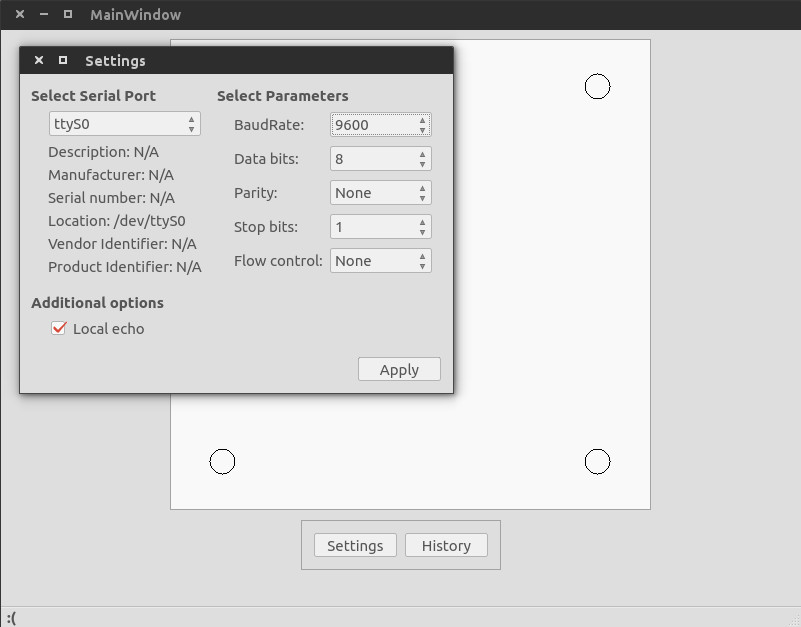
\includegraphics[width=.8\textwidth]{figures/UI}
			\end{center}
			\caption{UI of the program}
			\label{fig:ui}
		\end{figure}